% --- Template for thesis / report with tktltiki2 class ---
% 
% last updated 2013/02/15 for tkltiki2 v1.02

\documentclass[finnish]{tktltiki2}

% tktltiki2 automatically loads babel, so you can simply
% give the language parameter (e.g. finnish, swedish, english, british) as
% a parameter for the class: \documentclass[finnish]{tktltiki2}.
% The information on title and abstract is generated automatically depending on
% the language, see below if you need to change any of these manually.
% 
% Class options:
% - grading                 -- Print labels for grading information on the front page.
% - disablelastpagecounter  -- Disables the automatic generation of page number information
%                              in the abstract. See also \numberofpagesinformation{} command below.
%
% The class also respects the following options of article class:
%   10pt, 11pt, 12pt, final, draft, oneside, twoside,
%   openright, openany, onecolumn, twocolumn, leqno, fleqn
%
% The default font size is 11pt. The paper size used is A4, other sizes are not supported.
%
% rubber: module pdftex

% --- General packages ---

\usepackage[utf8]{inputenc}
\usepackage[T1]{fontenc}
\usepackage{lmodern}
\usepackage{microtype}
\usepackage{amsfonts,amsmath,amssymb,amsthm,booktabs,color,enumitem,graphicx}
\usepackage[pdftex,hidelinks]{hyperref}
\usepackage{algpseudocode}
\usepackage{float}
\usepackage{subcaption}

% Automatically set the PDF metadata fields
\makeatletter
\AtBeginDocument{\hypersetup{pdftitle = {\@title}, pdfauthor = {\@author}}}
\makeatother

% --- Language-related settings ---
%
% these should be modified according to your language

% babelbib for non-english bibliography using bibtex
\usepackage[fixlanguage]{babelbib}
\selectbiblanguage{finnish}

% add bibliography to the table of contents
\usepackage[nottoc]{tocbibind}
% tocbibind renames the bibliography, use the following to change it back
\settocbibname{Lähteet}

% --- Theorem environment definitions ---

\newtheorem{lau}{Lause}
\newtheorem{lem}[lau]{Lemma}
\newtheorem{kor}[lau]{Korollaari}

\theoremstyle{definition}
\newtheorem{maar}[lau]{Määritelmä}
\newtheorem{ong}{Ongelma}
\newtheorem{alg}[lau]{Algoritmi}
\newtheorem{esim}[lau]{Esimerkki}

\theoremstyle{remark}
\newtheorem*{huom}{Huomautus}


% --- tktltiki2 options ---
%
% The following commands define the information used to generate title and
% abstract pages. The following entries should be always specified:

\title{Vakaa avioliitto -ongelma}
\author{Anis Moubarik}
\date{\today}
\level{Tutkielma}
\abstract{Vakaa avioliitto -ongelma on tilanne jossa on kaksi erillistä samansuuruista joukkoa joilla on jonkilainen mieltymys vastakkaisen joukon alkioista, tilannetta kutsutaan avioliittopeliksi. Tutkielmassa esitellään vakauden määritelmä ja sen vaikutuksia pareihin ja pariutuksiin ja kuinka näitä vakaita pariutuksia löydetään avioliittopeleistä. Näiden ohella esitellään Gale--Shapley-algoritmi, joka tuottaa vakaan pariutuksen jokaiselle avioliittopelille.

Tutkielma käy läpi myös yleisimpiä muunnoksia alkuperäiseen ongelmaan, kuten erisuuruiset joukot ja parien kieltäminen, jotka johdattelevat oikean maailman sovelluksiin. Sovelluksista esitellään elinluovutus tapaukset, koulujen opiskelijavalinnat sekä opetussairaaloiden ja lääkettieteen opiskelijoiden pariutus. 

Lopuksi käydään läpi strategioita sekä koalitioita avioliittopeleissä. Kuinka ne vaikuttavat pariutukseen ja parantavatko strategiat niitä käyttävien alkioiden pareja, kuinka koalitiot voivat manipuloida Gale--Shapley-algoritmiä ja onko petos kannattavaa koalitioissa.}

% The following can be used to specify keywords and classification of the paper:

\keywords{vakaa pariutus, avioliittopeli, Gale--Shapley-algoritmi}
\classification{
\textbf{Theory of computation} $\rightarrow$ \textbf{Algorithmic game theory}; \emph{Mathematics of computing} $\rightarrow$ \emph{Combinatoric problems;}} % classification according to ACM Computing Classification System (http://www.acm.org/about/class/)
                  % This is probably mostly relevant for computer scientists

% If the automatic page number counting is not working as desired in your case,
% uncomment the following to manually set the number of pages displayed in the abstract page:
%
% \numberofpagesinformation{16 sivua + 10 sivua liitteissä}
%
% If you are not a computer scientist, you will want to uncomment the following by hand and specify
% your department, faculty and subject by hand:
%
% \faculty{Matemaattis-luonnontieteellinen}
% \department{Tietojenkäsittelytieteen laitos}
% \subject{Tietojenkäsittelytiede}
%
% If you are not from the University of Helsinki, then you will most likely want to set these also:
%
% \university{Helsingin Yliopisto}
% \universitylong{HELSINGIN YLIOPISTO --- HELSINGFORS UNIVERSITET --- UNIVERSITY OF HELSINKI} % displayed on the top of the abstract page
% \city{Helsinki}
%


\begin{document}

% --- Front matter ---

\maketitle        % title page
\makeabstract
\tableofcontents  % table of contents
\newpage          % clear page after the table of contents


% --- Main matter ---

\section{Johdanto}
Vakaa avioliitto -ongelma (\emph{stable marriage problem}) sivuaa kombinatoriikkaa ja peliteoriaa. Ongelma on seuraava: olkoon olemassa tilanne, jossa on $n$ miestä ja $n$ naista ja miehet ovat pistäneet naiset järjestykseen mieluisimmasta parista huonoimpaan ja jokainen nainen on pistänyt miehet vastaavaan järjestykseen, tilannetta kutsutaan \emph{avioliittopeliksi}. \emph{Pari} on tässä kontekstissa siis mies-nais pari, tätä kutsutaan myös \emph{avioliitoksi}. Tehtävänä on pariuttaa miehet ja naiset niin, että ei ole olemassa kahta vastakkaisen sukupuolen henkilöä, jotka olisivat mielummin pari keskenään kuin pysyisivät avioliitossaan nykyisessä pariutuksessa. Avioliitot ovat vakaita, kun näitä \emph{estepareja} ei esiinny. Pariutus on joukko pareja ja parit voidaan pariuttaa Gale--Shapley-algoritmilla, joka esitellään myöhemmin. Vakaassa pariutuksessa on siis tarkoitus pariuttaa kahden joukon alkiot niin että jokin kriteeri täyttyy, alkuperäisessä vakaa avioliitto -ongelmassa tuo kriteeri on parien vakaus suhteessa alkioiden mieltymyksiin.

Ongelmalla on monia käytännön sovelluksia. Se voidaan yleistää kaikkiin \emph{kaksipuolisiin markkinoihin} (\emph{two-sided markets}), joissa eettisistä tai laillisista syistä ei käytetä vaihtovälineenä rahaa. Kaksipuolisilla markkinoilla tarkoitetaan tilannetta, jossa on olemassa alusta, joka palvelee kahta erillistä ryhmää, jotka toimittavat toisilleen hyödykkeitä. Hyviä esimerkkejä ovat: elinluovuttajat ja vastaanottajat, työntekijät ja työnantajat sekä opiskelijat ja korkeakoulut.

Elinluovutusten tapauksessa haastena on, luovuttaja-potilas kaksikoiden yhteensopimattomuus. Vakaa avioliitto -ongelman ratkaisuja voidaan käyttää elinluovutuksissa, esimerkiksi jos on olemassa kaksikot $A$, $B$ ja $C$, eli jokainen kaksikoista sisältää luovuttajan ja potilaan, mutta syystä tai toisesta elin ei sovi potilaalle. Tässä esimerkissä voidaan soveltaa ratkaisuja ja saada vakaita pariutuksia potilaitten ja luovuttajien välille. Oletetaan, että $A$:n luovuttaja sopii $B$:lle, $B$:n $C$:lle ja $C$:n $A$:lle, nyt saadaan ketju ja vakaa pariutus, jossa jokainen potilas saa uuden elimen. Näitä \emph{kaksipuolisia pariutusmarkkinoita} tutkitaan tutkielmassa.

Gale ja Shapley esittivät vuonna 1962 ilmestyneessä artikkelissa \cite{gale62a} algoritmin alkuperäiselle ongelmalle, joka löytää yhden vakaan pariutuksen jokaiselle olemassa olevalle avioliittopelille. Jokaisella avioliittopelillä on siis vähintään yksi vakaa pariutus. Algoritmi toimii oletuksena miehet kosii, naiset hylkää periaatteella. Tämä antaa kosijalle, tässä tapauksessa siis miehille, aina parhaan mahdollisen parin mitä he voivat pelin kontekstissa saada. Naisten kosiessa roolit tietysti vaihtuvat ja pariutukset ovat silloin naisille optimoituja.
Avioliittopelien strategiat ovat peliteorian osa-alue ja se tulee esille, kun joukkojen alkiot käyttävät koalitioita ja strategoita vääristelemällä mieltymyksiään saadakseen edun pariutuksessa. Tähän vääristelyyn Gale--Shapley-algoritmi ei osaa puuttua ja se nostaakin kysymyksiä kuinka siihen pitäisi reagoida ja miten ylipäätään alkiot vääristelystä eri tapauksissa hyötyvät, jos hyötyvät ollenkaan.

Alkuperäiseen avioliitto-ongelmaan on pieniä variaatioita, kuten erisuuruiset joukot ja alkioiden hyvin erilaiset mieltymykset, eli tapaukset joissa he eivät halua pariutua tietyn henkilön kanssa ollenkaan. Näissä tapauksissa vakauden määritelmää muokataan niin että pariutukset joissa alkio on ilman paria voi olla myös vakaa. Erisuuruisten joukkojen tapauksessa suuremman joukon alkioista jää pariuttamatta suuremman ja pienemmän joukon alkioiden lukumärään erotuksen verran alkioita. Näitä variaatioita varten esitellään myös ratkaisut, jotka tuottavat vakaita pariutuksia.

\section{Vakaat pariutukset}
Olkooon $M$ \emph{miesten} joukko ja $N$ naisten joukko, missä $|M| = |N| = n$. Avioliitosta tai parista puhuttaessa tarkoitetaan sillä paria $(m, n) \in M \times N$. Avioliittopelissä jokaisella joukkojen alkiolla on mieltymykset toisen joukon alkioista parhaimmasta kumppanista huonoinpaan. Kuvassa \ref{pari} on esimerkki parista, joukoista $N$ ja $M$.

\begin{figure}[t]
	\begin{subfigure}{.6\textwidth}
	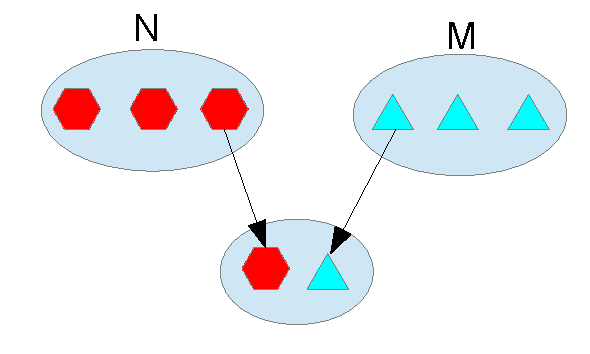
\includegraphics[scale=0.6]{paritutk}
	\caption{Yksi mahdollinen pari joukoista $M$ ja $N$}
	\label{pari}
	\end{subfigure}
	\begin{subfigure}{.3\textwidth}
	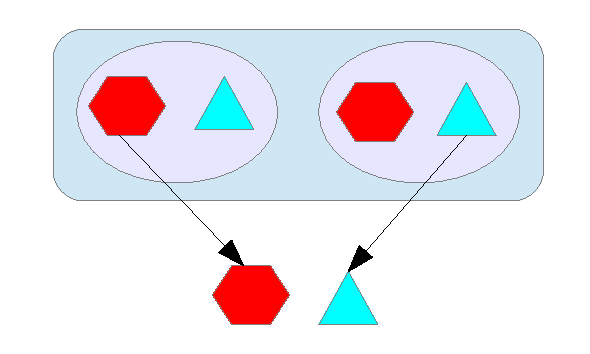
\includegraphics[scale=0.6]{vakaatutk}\label{epävakaa}
	\caption{Kuva epävakautta aiheuttavasta kaksikosta}
	\label{epävakaus}
	\end{subfigure}
	\caption{}
\end{figure}


Olkoon $M = \{m_1, m_2, m_3\}$ ja $N = \{n_1, n_2, n_3\}$. Mieltymykset voidaan kuvata esimerkiksi taulukossa. Järjestys taulukossa \ref{mieltymyksettaul} on vasemmalta oikealle laskevassa järjestyksessä, eli esimerkiksi miehelle $m_1$ miellyttävin pari olisi $n_2$. Henkilön mieltymyksia kuvaavaa järjestystä kutsutaan mieltymyslistaksi (\emph{preference list}), jossa toisen joukon alkiot ovat mieltymysjärjestyksessä.

\begin{table}[t]
\centering
	\begin{tabular}{ l | *{2}{c} r }
	 &  \\
	 \hline
 	 $m_{1}$ & $n_{1}$ & $n_{3}$ & $n_{2}$ \\
 	 $m_{2}$ & $n_{1}$ & $n_{2}$ & $n_{3}$ \\
 	 $m_{3}$ & $n_{3}$ & $n_{1}$ & $n_{2}$ \\
	\end{tabular}
	\quad
	\begin{tabular}{ l | *{2}{c} r }
	 &  \\
	 \hline
 	 $n_{1}$ & $m_{1}$ & $m_{2}$ & $m_{3}$ \\
 	 $n_{2}$ & $m_{2}$ & $m_{1}$ & $m_{3}$ \\
 	 $n_{3}$ & $m_{3}$ & $m_{2}$ & $m_{1}$ \\
	\end{tabular}
	\caption{Miesten ja naisten mieltymykset}
	\label{mieltymyksettaul}
\end{table}

Mieltymyksiä voidaan myös kuvata transitiivisella relaatiolla $>$. Esimerkiksi miehen $m_1$ mieltymykset voidaan esittää seuraavasti: $n_2 >_{m_1} n_1 >_{m_1} n_3$, relaatio on myös transitiivinen eli $n_2 >_{m_1} n_3$ pätee.

Pariutus $\mu$ on joukko $\mu \subseteq M \times N$, joka tulkittuna funktioksi $\mu : M \mapsto N$ on bijektio. Alkion $m$ paria pariutuksessa $\mu$ merkitään seuraavasti $p_{\mu}(m)$.

\begin{maar}
Pariutus $\mu$ on \emph{vakaa}, jos ei ole olemassa kaksikkoa $m_1$ ja  $n_2$, jolle
\begin{enumerate}
	\item $n_2 >_{m_{1}} p_{\mu}(m_1)$, ja
	\item $m_1 >_{n_{2}} p_{\mu}(n_2)$
\end{enumerate}


Kuvassa \ref{epävakaus} on pariutus, jossa on kaksi paria. Ensimmäisen parin nainen ja toisen parin mies pitävät toisistaan enemmän kuin omista pareistaan ja tämä aiheuttaa epävakautta.

\begin{ong}[Vakaa pariutus]
Vakaa pariutus joukoille $N$ ja $M$.
\end{ong}
\end{maar}

Myöhemmin esitellään teoreema, jonka mukaan jokaisesta avioliittopelistä löytyy ainakin yksi vakaa pariutus. Ensin kuitenkin esittellään algoritmi joka tarkastaa onko jokin mielivaltainen pariutus vakaa.
\begin{alg}\cite[s. 8]{gusfield1989stable}
Olkoon $m \in M$ ja $n \in N$ ja $\mu$ pariutus.
\begin{enumerate}
	\item Kaikilla $n$ siten että $m$ suosii naista $n$ enemmän kuin omaa paria $p_{\mu}(m)$, jos $n$ suosii miestä $m$ enemmän kuin omaa paria $p_{\mu}(n)$, ilmoitetaan että pariutus $\mu$ ei ole vakaa.
	\item Jos yhtään tälläistä paria ei löydetä ilmoitetaan, että pariutus $\mu$ on vakaa.
\end{enumerate}
\end{alg}

Etsitään tapauksia jossa mies suosii naista enemmän kuin omaa pariaan pariutuksessa $\mu$,
jos löytyy tälläinen mies, tarkistetaan suosiiko nainen häntä enemmän kuin omaa pariaan pariutuksessa, jos tämä pitää paikkansa ei pariutus voi olla vakaa.
Huonoimmassa tapauksessa käydään läpi kaikki miehet ja kaikki paitsi yksi naista, eli $x\cdot(x-1)$, tästä saadaan aikavaativuudeksi $O(x^2)$.

\subsection{Ylivallat}
Pariutuksilla ja pareilla on erilaisia ominaisuuksia. Paras-miehelle pari on pari, jossa mies saa haluamansa naisen ja vastaavasti paras-naiselle pari on pari, jossa nainen saa haluamansa miehen. Pariutuksissa voi esiintyä jommankumman joukon ylivaltaa, jos kaikilla $j \in N$, $j$ saavat haluamansa parin, tätä kutsutaan $N$-joukon ylivallaksi ja samoin kaikilla $i \in M$, $i$ saavat haluamansa parin, tällöin se on $M$-joukon ylivalta. Joskus ylivaltoja kutsutaan myös \emph{nais}- tai \emph{miesylivallaksi}. Jos ylivaltaa ei synny pariutuksessa, voidaan pariutusta kutsua ylivaltavapaaksi.
Päinvastoin jos mies tai nainen saa huonoimman tai vähiten haluamansa parin, kutsutaan sitä \emph{huonoin-naiselle} tai -\emph{miehelle} pariksi. Samoin paria kutsutaan huonoin-naiselle tai -miehelle pariksi jos kaikki jommankumman joukon alkioista saavat vähiten haluamansa parit.

\section{Gale--Shapley-algoritmi}
Avioliittopelistä löytyy aina ainakin yksi vakaa pariutus. Gale--Shapley-algoritmi on yksinkertainen algoritmi, joka tuottaa vakaan parituksen avioliittopelille. Seuraavaksi esitellään algoritmi ja näytetään, että se päättyy aina.
\begin{alg} \cite[s. 13]{gale62a} \label{gsalg}.
\begin{enumerate}
	\item Miehet aloittavat kosimalla mieltymyksiltään parasta naista.
	\item Naiset hylkäävät kaikki paitsi parhaiten sijoitetun miehen.
	\item Nainen ei hyväksy miestä vaan jättää miehen \emph{langan} päähän siltä varalta että parempi mies kosisi häntä
	\item Hylätyt miehet kosivat mieltymyksiltään toisiksi parasta naista.
	\item Naiset hylkäävät kaikki paitsi parhaan vaihtoehdon
	\item Niin kauan kuin joku naisista ei ole saanut kosintaa, tulee hylkäyksiä ja uusia kosintoja. Lopuksi jokaista naista on kosittu, koska mies ei voi kuin kerran kosia samaa naista.
	\item Viimeinen nainen on saanut kosinnan ja kosimisvaihe on päättynyt. Jokainen nainen hyväksyy langan päässä olevan kosijan
\end{enumerate}
\end{alg}


\begin{lau}
Algoritmi \ref{gsalg} pysähtyy kaikilla söytteillä
\begin{proof}
Mies ei voi jäädä ilman paria. Nainen voi hylätä vain jos hänellä on langan päässä mies, nainen ei voi ensimäisellä kierroksella hylätä miestä (kierroksella tarkoitetaan siis yhden miehen kosintaa ja naisen vastausta siihen), ja kun hänellä on langan päässä mies hänestä ei tule missään vaiheessa vapaata algoritmin suorittamisessa.
Jos viimeinen nainen jota kositaan hylkää miehen, tarkoittaisi tämä sitä, että jokaisella naisella olisi mies jo langan päässä. Mutta naisia ja miehiä on sama määrä ja yksikään mies ei voi olla kahden naisen langan päässä, niin jokainen miehistäkin pitäisi olla lankojen päässä, mikä on ristiriita.
Jokaisella kierroksella mies kosii tasan yhtä naista, ja koska mies voi kosia koko algoritmin suorituksen aikana jokaista naista maksimissaan kerran on kierroksien määrä huonnoimassa tapauksessa $n^2$.
\end{proof}
\end{lau}

Otetaan esimerkiksi taulukko \ref{mieltymyksettaul}, kierroksia tulee yhteensä 4, jos mieltymykset olisivat erilaiset voisi kierrosten määrä olla parhaassa tapauksessa 3, eli jokaisella kierroksella nainen hyväksyy kosivan miehen ilman hylkäyksiä. Huonoimmassa tapauksessa miesten listalta vasta viimeiset naiset hyväksyvät ja kierrosten lukumäärä on silloin 9.
Algoritmi \ref{gsalg} on siis päättyvä, mutta onko pariutukset aina vakaita?
Todistetaan tämä.
\begin{lau}
Algoritmin \ref{gsalg} tuottamat pariutukset ovat aina vakaita.
\begin{proof}\cite[s. 588]{gale62a}
Olkoon olemassa mies $m$ ja nainen $n$ ja oletetaan, että he eivät ole pari pariutuksessa $\mu$. Oletetaan myös, että $n >_{m} p_{\mu}(m)$. Miehen $m$ on siis jossain vaiheessa algoritmiä kosia naista $n$ ja naisen $n$ on pitänyt jossain vaiheessa hylkää $m$ paremman miehen tieltä. Siis $n$ suosii omaa pariaan pariutuksessa $\mu$ miehen $m$ sijaan, eikä epävakautta voi syntyä.
\end{proof}
\end{lau}
Algoritmi tuottaa tälläisenaan miehelle optimaalisia tuloksia, eli tällä algoritmilla tuotettu pariutus on kyseiselle miehille paras mahdollinen mitä he siinä kyseisessä avioliittopelissä tulevat saamaan.
Naisille optimaalisia tuloksia voidaan saada, kun osat vaihdetaan päittäin algoritmissä.

\begin{esim}
	Katsotaan 3 kokoista avioliittopeliä ja mieltymyslistaa taulukosta \ref{mieltymyksettaul}.
	
	Yksi mahdollinen suoritus olisi seuraava: mies $m_1$ aloittaa kosimalla naista $n_1$ (nainen hyväksyy); mies $m_2$ kosii naista $n_1$ (nainen hylkää, hänellä on parempi mies langan päässä); mies $m_3$ kosii naista $n_3$ (nainen hyväksyy); mies $m_2$ kosii uudestaan, nyt listalla toista olevaa naista $n_2$ (nainen hyväksyy). Jokaista naista on kosittu ja jokaisella on joku mies langan päässä, kosinta on päättynyt ja naiset hyväksyvät langan päässä olevan miehen lopullisesti. Lopullinen vakaa pariutus on seuraava $\{(m_1, n_1), (m_2, n_2), (m_3, n_3)\}$.
\end{esim}

\section{Vakaitten pariutusten joukko}
Gale-Shapley algoritmi tuottaa meille yhden vakaan pariutuksen, mutta niitä voi olla enemmän.
Olkoon $\mu$ ja $\delta$ pariutukset. Henkilö $x$ suosii pariutusta $\mu$ pariutukseen $\delta$ nähden, jos $x$ suosii enemmän pariaan $\mu$ pariutuksessa kuin $\delta$ pariutuksessa. Henkilölle voi olla myös välinpitämätön pariutuksista, jos molemmat antavat hänelle yhtä hyvän parin.

\begin{lau} \cite[p. 18]{gusfield1989stable}\label{lause-guspref}
	Olkoon $\mu$ ja $\delta$ vakaita pariutuksia, ja oletetaan että $m$ ja $n$ ovat pari pariutuksessa $\mu$ muttei $\delta$:ssa. Nyt jompikumpi henkilöistä $m$ ja $n$ suosii pariutusta $\mu$ enemmän kuin pariutusta $\delta$ ja toinen pariutusta $\delta$ enemmän kuin pariutusta $\mu$.
\begin{proof} \cite[s. 18]{gusfield1989stable}
Olkoon $\mathcal{X}$ ja $\mathcal{Y}$ naisten ja miesten joukot jotka pitävät pariutusta $\mu$ parempana, kuin pariutusta $\delta$. Vastaavasti joukot $\mathcal{X}'$ ja $\mathcal{Y}'$ pitävät pariutusta $\delta$ parempana, kuin pariutusta $\mu$.

Pariutuksessa $\mu$ ei voi olla paria $(m, n)$ missä $m \in \mathcal{X}$ ja $n \in \mathcal{Y}$, koska tämä pari estäisi pariutuksen $\delta$. Joten jokaisella miehellä joukossa $\mathcal{X}$ on $\mu$-pari (\emph{$\mu$-partner}) joukosta $\mathcal{Y'}$, näin ollen $|\mathcal{X}| \leq |\mathcal{Y'}|$.

Samoin pariutuksessa $\delta$ ei voi olla paria $(m, n)$ missä $m \in \mathcal{X}'$ ja $n \in \mathcal{Y}'$, koska tämä pari estäisi pariutuksen $\mu$. Joten jokaisella miehellä joukossa $\mathcal{X}'$ on $\delta$-pari joukosta $\mathcal{Y}$, näin ollen $|\mathcal{X}'| \leq |\mathcal{Y}|$.

Huomataan, että $|\mathcal{X}| + |\mathcal{X}'| = |\mathcal{Y}| + |\mathcal{Y}'|$, koska vasen puoli on miesten lukumäärä ja oikea puoli naisten lukumäärä, joilla en eri parit kyseisissä pariutuksissa. Tästä seuraa $|\mathcal{X}'| = |\mathcal{Y}|$ ja $|\mathcal{X}| = |\mathcal{Y}'|$. Näin ollen jokaisella miehellä joukossa $\mathcal{X}'$ on $\mu$-pari joukosta $\mathcal{Y}$, ja koska jokaisella miehellä joukossa $\mathcal{X}$ on $\mu$-pari joukosta $\mathcal{Y}'$ lemma \ref{lause-guspref} pitää paikkansa.
\end{proof}
\end{lau}

Tästä seuraa korollaari \ref{eqkor}.

\begin{kor}\cite[s. 18]{gusfield1989stable}\label{eqkor}
Jos $\mu$ ja $\delta$ ovat vakaita pariutuksia samalle avioliittopelille, niin henkilöiden määrä jotka suosivat pariutusta $\mu$ on sama kuin henkilöiden määrä jotka suosivat pariutusta $\delta$.
\end{kor}

Esitellään notaatiota (mies-orientoituneille) ylivalloille. Pariutus $\mu$ dominoi pariutusta $\delta$, jos jokainen mies saa vähintään yhtä hyvän parin pariutuksessa $\mu$ kuin pariutuksessa $\delta$, merkitään sitä seuraavasti $\mu \preceq \delta$.
Jos miesten kosiessa pariutuksessa on miesylivalta se tarkoittaa sitä, että naisten kosiessa on pariutukseen muodostuttava naisylivalta, jota merkitään seuraavasti $\mu \succeq \delta$. Olkoon $\mathcal{M}$ kaikkien pelin vakaiden pariutusten joukko avioliittopelissä. $(\mathcal{M}, \preceq)$ on osittain järjestetty joukko.
Seuraava korollaari seuraakin lauseesta \ref{lause-guspref}.

\begin{kor}\cite[s. 19]{gusfield1989stable}
Miehen näkökulmasta pariutus $\mu$ dominoi pariutusta $\delta$, joss pariutus $\delta$ dominoi pariutusta $\mu$ naisten näkökulmasta. \emph{Nais-orientoitunut} ylivalta relaatio on käänteinen, merkinnällä $\succeq$, mies-orientoituneeseen nähden. Tämä on myös osittain järjestetty joukko ja se merkitään seuraavasti $(\mathcal{M}, \succeq)$. 
\end{kor}

\subsection{Vakaitten pariutusten määrä}
Näytetään, että vakaita pariutuksia on eksponentiaalinen määrä. Jos halutaan löytää kaikki mahdolliset vakaat pariutukset joudutaan käyttämään brute-force-algoritmia, ja aikavaativuus on tällöin eksponentiaalinen.

\begin{lem} \cite[s. 23]{gusfield1989stable} \label{lemma-koko}
Olkoon olemassa vakaat avioliittopelit kooltaan $m$ ja $n$ ja vastaavasti olkoon $x$ ja $y$ vakaiden pariutuksien määrä avioliittopeleissä. On olemassa peli jonka koko on $m \cdot n$, jolla on vähintään $\max(xy^m, yx^n)$ vakaata pariutusta.

\begin{proof}\cite[s. 23]{gusfield1989stable}
Merkitään miehiä ja naisia lemman \ref{lemma-koko} avioliittopeleissä seuraavasti, $a_1,...,a_{m}, c_1,...,c_{m}$ ja $b_1,...,b_{n}, d_1,...,d_{n}$. Tarkistellaan $mn$ kokoista peliä, missä
\begin{enumerate}
\item miehet on merkitty seuraavasti $(a_i,b_j), i = 1,...,m, j = 1,...,n$,
\item naiset on merkitty seuraavasti $(c_i,d_j), i = 1,...,m, j = 1,...,n$,
\item mies $(a_i, b_j)$ suosii naista $(c_k, d_l)$ enemmän kuin naista $(c_k',d_l')$, jos $b_j$ suosii enemmän naista $d_l$ kuin naista $d_{l'}$, tai $l = l'$ ja $a_i$ suosii naista $c_k$ enemmän kuin naista $c_{k'}$,
\item nainen $(c_i, d_j)$ suosii miestä $(a_k, b_l)$ enemmän kuin miestä $(a_{k'}, b_{l'})$, jos $d_j$ suosii miestä $b_l$ enemmän kuin miestä $b_{l'}$, tai jos $l = l'$ ja $c_i$ suosii miestä $a_k$ enemmän kuin miestä $a_{k'}$.
\end{enumerate}

Olkoon $\mu_{1},...,\mu_{n}$ mikä tahansa sarja vakaita pariutuksia avioliittopelissä, jonka koko on $m$, ja olkoon $\mu$ mikä tahansa vakaa pariutus avioliittopelissä, jonka koko on $n$. Mahdollisten pariutusten määrä pariutuksille $\mu_{1},...,\mu_{n}$ ja $\mu$ on $yx^n$. Väitetään, että kuvaus

$(a_i, b_j) \longrightarrow (p_{\mu_{j}}(a_i),p_{\mu}(b_j))$

on vakaa pariutus yhdistetyssä avioliittopelissä.

Tämä kuvaus on pariutus , koska molemmat, $\mu_j$ ja $\mu$ ovat pariutuksia. Oletetaan, että tässä pariutuksessa on seuraava estepari $((a,b),(c,d))$. Nyt seuraavista ehdoista, joko 1. ja 2. tai 3. ja 4. täytyy olla voimassa.

\begin{enumerate}
	\item $b$ suosii enemmän henkilöä $d$ kuin $p_\mu(b)$,
	\item $d = p_\mu(b)$ ja $a$ suosii enemmän henkilöä $c$ kuin $p_{\mu_{j}}(a)$,
	\item $d$ suosii enemmän henkilöä $b$ kuin $p_\mu(d)$,
	\item $b = p_\mu(d)$ ja $c$ suosii enemmän henkilöä $a$ kuin $p_{\mu_{j}}(c)$.
\end{enumerate}

Neljästä mahdollisesta kombinaatiosta, kombinaatio ehdoilla 1 ja 3 on esteenä pariutuksen $\mu$ vakaudelle, kombinaatio ehdoilla 2 ja 4 on esteenä pariutuksen $\mu_j$ vakaudelle ja muut kombinaatiot ovat yhteensopimattomia.

Näin ollen väittämä on oikeutettu, ja on näytetty avioliittopeli missä on vähintään $yx^n$ vakaata pariutusta. Samalla tavoin, vaihtamalla rooleja alkuperäisissä avioliittopeleissä, vahvistetaan vastaava tulos määrälle $xy^m$.
\end{proof}
\end{lem}

\begin{lem}\cite[p. 24]{gusfield1989stable}
Jokaiselle $n \geq 0$, missä $n$ on kahden potenssi, on olemassa vakaa avioliittopeli jonka koko on $n$ ja sisältää vähintään $2^{n-1}$ vakaata pariutusta
\end{lem}
\begin{proof}
Todistus induktiolla. Kun pelin koko on 1, eli alkioiden lukumäärä on 1, niin $n = 2^0$ triviaali tapaus, eli vakaita pariutuksia on yksi. Oletetaan tulos todeksi tapauksessa $n = 2^k$, käytetään lemmaa \ref{lemma-koko}, missä $i = 2$, avioliittopeli jonka koko on siis 2. Molemmat mahdolliset pariutukset ovat vakaita, joten $x = 2$ ja induktio-oletuksen mukaan $y = 2^{2^{k-1}}$. Joten lemman \ref{lemma-koko} perusteella on olemassa peli jonka koko on $2 \cdot 2^k = 2^{k+1}$, jolla on vähintään $\max(2 \cdot (2^{2^{{k}}-1})^2, 2^{2^{k}-1} \cdot 2^{2^{k}})) = 2^{2^{k+1}-1}$ vakaata paritusta.
\end{proof}

\section{Laajennettu Gale--Shapley-algoritmi}
Tämän algoritmin tarkoituksena on yksinkertaistaa vakaa avioliitto -ongelman eri ongelmakohtien ratkomista. Algoritmi on suunniteltu tekemään enemmän, kuin vain löytää yksi vakaa pariutus. Laajennettua algoritmia tullaan tarvitsemaan vakaa avioliitto -ongelman sovelluksissa, erityisesti tapauksissa, joissa parille on kahdesta alkiosta yhdentekevää kumman kanssa pariutuu, tämä tulee esille myöhemmässä kappaleessa. Algoritmi sieventää alkioiden mieltymyslistoja poistamalla pareja, jotka eivät kuulu mihinkään vakaaseen pariutukseen. Poistamalla pari $(m, n)$ tarkoitetaan sillä sitä että $n$ poistetaan miehen $m$ mieltymyslistalta ja $m$ naisen $n$ listalta.

\begin{alg}\cite[s. 16]{gusfield1989stable}\label{alg2}
	\begin{enumerate}
		\item Alustetaan jokainen henkilö vapaaksi.
		\item Niin kauan kuin joku mies $m$ on vapaa,
		\item valitaan ensimmäinen nainen miehen listalta.
		\item Jos naisella $n$ on jo langan päässä mies $p$, vapautetaan $p$ ja asetetaan $m$ naisen $n$ langan päähän.
		\item Poistetaan jokainen pari $(m', n)$, missä $m'$ on $m$:n seuraaja $n$ mieltymyslistalla.
	\end{enumerate}
\end{alg}

Tässä algoritmissä, kun mies kosii naista kosinta hyväksytään aina. Koska jos naisella $n$ on jo langan päässä joku miellyttävämpi mies, kuin $m$ olisi pari $(m, n)$ poistettu.
Algoritmi pysähtyy, kun jokaisella naisella on jokin mies langan päässä. Huomataan myös, että algoritmin lopettaessa jokainen mies on listalla ensimmäisenä olevan naisen langan päässä ja jokaisella naisella taas langan päässä viimeisenä listalla oleva mies.

Kutsutaan algoritmin tuottamaa mieltymyslistaa, jossa miehet kosivat, \emph{mies-orientoituneeksi Gale--Shapley listaksi} tai \emph{MGS-listaksi}. Vastaavasti, jos miesten ja naisten roolit algoritmissä vaihdetaan kutsutaan tuotettua listaa \emph{NGS-listaksi}. Jos otetaan henkilön MGS- ja NGS-listan leikkaus saadaan tulokseksi GS-lista.

\begin{lau}\cite[s. 17]{gusfield1989stable}\label{laajlause}
	Annetulle avioliittopelille pätee, että
	\begin{itemize}
		\item kaikki vakaat pariutukset ovat GS-listassa,
		\item yksikään pari, joka ei ole GS-listalla ei voi estää pariutusta GS-listalta,
		\item mies-optimaalisissa (vastaavasti nais-optimaalisissa) pariutuksissa jokainen mies on pariutettu ensimmäisen (vastaavasti viimeisen) naisen kanssa hänen GS-listalta ja jokainen nainen viimeisen (vastaavasti ensimmäisen) miehen kanssa naisen listalta.
	\end{itemize}
\end{lau}

\begin{esim}
	Taulukossa \ref{mieltymyksettaul} jokaisen henkilön GS-lista sisältää vain hänen vakaan parinsa, sillä molemmat mies- ja nais-optimaaliset pariutukset ovat samat tässä tapauksessa.
\end{esim}


\section{Erisuuruiset joukot}
Esitellään nyt ongelman pieni variaatio, missä joukot jotka pitää pariuttaa, ovat erisuuria. Aiemmat tulokset pätevät muokattuina myös tässä tapauksessa. Oletetaan, että henkilö haluaa olla ennemmin naimisissa kuin naimaton.
Olkoon $M$ miesten joukko ja $N$ naisten joukko, ja $|M| = n_x < n_y = |N|$.

\begin{maar}
 Pariutus $\mu$ on epävakaa, jos on olemassa mies $m$ ja nainen $n$ siten että
\begin{enumerate}
	\item $m$ ja $w$ eivät ole pari pariutuksessa $\mu$,
	\item $m$ on joko ilman paria $\mu$:ssä tai suosii naista $w$ enemmän kuin pariaan pariutuksessa $\mu$, ja
	\item $w$ on joko ilman paria $\mu$:ssä tai suosii miestä $m$ enemmän kuin pariaan pariutuksessa $\mu$.
\end{enumerate}
\end{maar}

Jokainen vakaa pariutus koostuu $n_x$:stä järjestettyjä pareja, missä $n_x - n_y$ on naimattomien naisten määrä.

Käyttämällä mies-orientoitunutta Gale--Shapley-algoritmiä, päättyy  se niin että jokainen mies on langan päässä ja tuloksena oleva pariutus on vakaa. Pariutus on mies-optimaalinen ja $n_x - n_y$ naista jää parittomaksi.

Jos käytetään nais-orientoitunutta versiota laajennetusta algoritmistä päättyy se siihen, että jokaisella miehellä on langan päässä jokin nainen, ja pariutus on vakaa. Huomataan kuitenkin, että jokaisen pariuttamattoman naisen WGS-lista on tyhjä ja seurauksena lauseesta \ref{laajlause}(1) nämä naiset eivät voi olla pariutettuna missään vakaassa pariutuksessa \cite[s. 26]{gusfield1989stable}.

\begin{lau}\cite[p. 26]{gusfield1989stable}.
Erisuuruistem joukkojen avioliittopelissä, on olemassa vähintään yksi vakaa pariutus, jossa pienemmän joukon kaikki alkiot saavat parin.
\end{lau}
Jos avioliittopeli, jossa on erisuuruiset joukot tuottaa saman GS-listan kuin avioliittopeli, jossa on samansuuruiset joukot, niin molempien vakaat pariutukset ovat samoja.

Alkuperäistä algoritmiä \ref{gsalg} voidaan myös muokata yksinkertaisilla muutoksilla. Jos on olemassa $x$ määrä miehiä ja $y$ määrä naisia, ja $x > y$, muokataan algoritmin 6. kohtaa, kun $x$ määrä naisia on kosittu päätetään algoritmin suoritus siihen. Jos taas $x < y$, niin algoritmi toimii normaalisti.


\section{Parien kieltäminen}
Jos henkilön on mahdollista ilmoittaa, että yksi tai useampi ei kelpaa hänelle vastakkaisen sukupuolen joukosta, on hänen mieltymyslistansa aito osajoukko vastakkaisen sukupuolen joukosta. Näin ollen mies ja nainen voidaan pariuttaa ainoastaan jos he ovat hyväksyttäviä toisillensa.

Tässä tapauksessa vakaa pariutus voi olla osittainen, tarkoittaen että kaikkien henkilöiden ei tarvitse olla pariutettuna, jotta pariutus olisi vakaa.

\begin{maar}
Osittainen pariutus $\mu$ on epävakaa, jos on olemassa mies $m$ ja nainen $n$ siten että
\begin{enumerate}
	\item $m$ ja $n$ eivät ole pari pariutuksessa $\mu$, mutta molemmat hyväksyisivät toisensa,
	\item $m$ on joko pariuttamaton tai suosii naista $n$ enemmän kuin hänen pariaan pariutuksessa $\mu$,
	\item $n$ on joko pariuttamaton tai suosii miestä $m$ enemmän kuin hänen pariaan pariutuksessa $\mu$.
\end{enumerate} 
\end{maar}

Mieltymykset voidaan myös laajentaa koskemaan pariutuksia, eli henkilö suosii pariutusta jossa hänellä on pari verratuna pariutukseen jossa hän jää ilman paria. Käytetään samaa notaatiota, kuin parien mieltymyksissä, eli jos mies $m$ pitää pariutusta $\mu$ parempana kuin $\mu'$, niin merkitään sitä $\mu >_m \mu'$.

\begin{lau}
Avioliittopelissä, joka sallii parien kieltämisen on miehet ja naiset jaettu kahteen joukkoon -- niihin joilla on pari kaikissa pariutuksissa ja niihin joilla ei ole yhtään paria missään pariutuksessa.
\end{lau}

\begin{proof}\cite[p. 27]{gusfield1989stable}
Olkoon kaksi eri vakaata pariutusta $\mu$ ja $\delta$, määrittellään suunattu verkko $G = G(\mu, \delta)$, jossa solmu esittää yhtä henkilöä. Jokaiselle miehelle $m$ jolla on pari pariutuksessa $\mu$ on olemassa suunnattu kaari $m$:stä pariin $p_{\mu}(m)$. Ja jokaiselle naiselle $n$ jolla on pari pariutuksessa $\delta$ on olemassa suunnattu kaari $n$:stä pariin $p_{\delta}(n)$.
Jokaisella solmulla on verkossa $G$ enintään yksi tuleva ja lähtevä kaari.

Oletetaan nyt ristiriitaisesti, että $m$ on pariutettu naisen $n$ kanssa pariutuksessa $\mu$ muttei pariutuksessa $\delta$. On olemassa uniikki suunnaattu polku verkossa $G$ joka alkaa solmusta $m$ ja koska jokaisella solmulla on enintään yksi sisääntuleva kaari, ja $m$:llä on 0 sisääntulevaa kaarta, polku ei voi olla syklinen. Joten polun on päätyttävä mieheen joka on pariutettu $\delta$:ssa muttei $\mu$:ssa, eli $m$ suosii pariutusta $\delta$ ennemmin kuin pariutusta $\mu$, tai naiseen $n$ joka on pariutettu $\mu$:ssa muttei $\delta$:ssa $n$ suosii siis pariutusta $\mu$ ennemmin kuin pariutusta $\delta$.

Mutta koska $m$ suosii pariutusta $\mu$ pariutuksen $\delta$ sijaan, seuraa lauseen \ref{lause-guspref} mukaan, että $n$ suosii pariutusta $\delta$ pariutuksen $\mu$ sijaan, ja lausetta \ref{lause-guspref} soveltamalla polkuun huomataan, että jokainen mies suosii pariutusta $\mu$ ja jokainen nainen pariutusta $\delta$. Joten kahdesta mahdollisesta reitistä, jossa polku voisi päättyä johtaa molemmat ristiriitaan.
\end{proof}

\section{Parien yhdentekeväisyys}
Parien yhdentekeväisyydellä tarkoitetaan tilanteita, joissa alkioiden mieltymyslistat eivät ole ehdottomasti sijoitettuja, eli alkio voi pitää yhdestä alkiosta yhtä paljon kuin toisesta. Toisin sanoen alkiolle on yhdentekevää kumman parin kanssa hänet pariutetaan.

Täsmennetään vakauden määritelmää. Ensimmäinen täsmennys on, jos on olemassa nainen ja mies, jotka eivät ole pari, mutta pitävät toisistaan enemmän tai yhtäpaljon kuin omista pareistaan kyseisessä pariutuksessa, on pariutus epävakaa. Jos pariutus on edellisen kriteerin perusteella vakaa, kutsutaan sitä \emph{super-vakaaksi} (\emph{super-stable}) \cite{gusfield1989stable}. Tilanteessa jossa on olemassa täysi välinpitämättömyys ei voi löytyä yhtään super-vakaata pariutusta \cite[s. 29]{gusfield1989stable}.

Toinen, vapaamuotoisempi, täsmennys on seuraava: jos on olemassa mies ja nainen, jotka eivät ole pari, joista toinen pitää toisesta enemmän kuin omasta paristaan pariutuksessa ja toinen on vähintään välinpitämätön paristaan, on pariutus epävakaa. Jos pariutus on edellisen kriteerin perusteella vakaa, kutsutaan sitä \emph{vahvastivakaaksi} (\emph{strongly-stable}) \cite[s. 29]{gusfield1989stable}.

Laajennettua Gale--Shapley-algoritmia voidaan käyttää löytämään super- ja vahvasti-vakaita pariutuksia jokaiselle avioliittopelille, joka sallii välinpitämättömyyttä.

Algoritmi toimii niin, että miehet kosivat naisia listaltaan ja kun törmäävät tilanteeseen jossa hänellä on kaksi tai enemmän naista listallaan, joista hän on neutraali ja he ovat tasoissa, kosii hän kaikkia naisia samanaikaisesti. Jos nainen saa kosinnan poistetaan kaikki huonommat parit naisen listalta ja nainen miesten listoilta. Nainen voi kuitenkin pitää montaa miestä langan päässä, jos he ovat naisen listalla tasoissa. Kosinta vaihe voi jättää miesten listat tyhjiksi, joka tarkoittaa sitä että super- tai vahvaa-pariutusta ei löytynyt. Muussa tapauksessa jokainen mies on yhden tai useamman naisen langan päässä.

\section{Vakaa huonetoveri -ongelma}
Vakaa huonetoveri -ongelma (\emph{Stable Roommate Problem}) on yleistetty vakaa avioliitto -ongelma, missä on vain yksi joukko, josta jokainen henkilö pistää toisensa mieltymys järjestykseen. Mieltymysten perusteella tehdään pariutukset, kuten vakaa avioliitto -ongelmassa. Vakaa huonetoveri -ongelmaa käytetään elinluovutuksissa, joista puhutaan myöhemmin omassa kappaleessa.

Pariutus on tässäkin tapauksessa epävakaa, jos on olemassa kaksi henkilöä jotka olisivat mielummin keskenään yhdessä kuin omien pariensa kanssa. Käytetään parien notaatiossa aaltosulkuja tavallisten sulkujen sijaan seuraavasti, jos $x$ ja $y$ ovat parit niin sitä merkitään näin $\{x, y\}$. Aaltosulkuja käytetään, koska parit eivät ole järjestyksessä kuten alkuperäisessä avioliitto-ongelmassa \cite[s. 163]{gusfield1989stable}. Suurin ero tavalliseen vakaa avioliitto -ongelmaan on se, että vakaa huonetoveri -ongelmassa voi olla tilanteita joissa ei ole ainuttakaan vakaata pariutusta.

\begin{table}[H]
\begin{center}
	\begin{tabular}{ l | *{2}{c} r }
	 &  \\
	 \hline
 	 $1$ & $3$ & $2$ & $4$ \\
 	 $2$ & $1$ & $3$ & $4$ \\
 	 $3$ & $2$ & $1$ & $4$ \\
 	 $4$ & &mielivaltainen
	\end{tabular}
	\caption{Huonetoveri ongelman mieltymykset \cite[s. 164]{gusfield1989stable}}
	\label{room-table}
\end{center}
\end{table}

Taulukko \ref{room-table} edustaa peliä jossa ei ole yhtään vakaata pariutusta. Kolmessa mahdollisessa pariutuksessa on vastaavasti parit $\{1,4\}$, $\{2,4\}$, $\{3,4\}$ ja nämä ovat vastaavasti estetty seuraavilla pareilla: $\{1,2\}$, $\{2,3\}$, $\{3,1\}$.

Käydään algoritmin toiminta yleisellä tasolla läpi. 
\begin{alg}\label{srp1}
Merkintöjä poistetaan etenevästi mieltymyslistoilta kunnes jompikumpi päättävistä ehdoista toteutuu \cite[s. 165]{gusfield1989stable}.
\begin{enumerate}
	\item Jokin mieltymyslistoista tyhjenee tarkoittaen, että yhtäkään vakaata pariutusta ei ole kyseiselle pelille, tai
	\item jokainen lista on sievennetty yhteen merkintään, missä tapauksessa nämä merkinnät koostavat vakaan pariutuksen.
\end{enumerate}
\end{alg}

\section{Sovellukset}
\subsection{Elinluovutus}
Alkuperäisessä sovelluksessa molemmat osapuolet ovat aktiivisia parin haun osalta. Elinluovutusten yhteydessä päätösten tekeminen on yksipuolista sillä ainoa asia joka vaikuttaa parien vakauteen on elimen yhteensopivuus vastaanottajalle. Voi olla tilanne jossa $A$ haluaa luovuttaa elimen $A'$:lle ja $B$ luovuttaa $B'$:lle, mutta erinnäisten epäsopivuuksien takia eivät he voi luovuttaa toisilleen elintä. Jos luovuttajan $A$ elin sopii potilaalle $B'$ ja $B$:n elin sopii potilaalle $B'$ voidaan järjestää tilanne, jossa $A$ luovuttaa $B'$:lle ja $B$ luovuttaa $A'$:lle. Tästä syntyy eräänlaisia ketjuja tai \emph{syklejä} joilla saadaan jokaiselle osallistuvalle potilaalle elin ja näin ollen lyhennettyä elinjonotusta muille potilaille.
Esimerkiksi munuaistenluovutuksissa on olemassa kaksi lähdettä munuaisille siirtoa varten:
\begin{enumerate}
	\item Ruumis elinluovutukset, ja
	\item Elävät munuaisluovutukset sukulaisilta, puolisolta tai muilta luovuttajilta. \cite[s. 6]{NBERw10002}
\end{enumerate}

Algoritmiä \ref{srp1} ja vakaa huonetoveri -ongelmaa joudutaan kuitenkin hieman muokkaamaan tätä sovellusta varten. Alkio tai "henkilö" tässä tapauksessa on vastaanottaja-luovuttaja kaksikko, jotka eivät voi luovuttaa toisilleen, eli ${x, y}$ on neljän henkilön pari. Toinen muutos on tapaus jossa mikään elin ei sovi vastaanottajalle, jos näin käy pidetään häntä odotuslistalla kunnes sopiva löytyy. Jos on olemassa luovuttaja-vastaanottaja kaksikot ${A, A'}, {B, B'}, {C, C'}$, jotka haluavat luovuttaa toisillensa elimen, mutta eivät syystä tai toisesta voi, voidaan muodostaa vaihtosykli parien välille. Suora vaihtosykli ei aina kelpaa, koska esimerkiksi $A$:n elin voi sopia $B'$:lle, mutta $B$:n elin ei sovi kummallekkaan $A'$ tai $C'$:lle, jos näin tapahtuu asetetaan $A'$ ja $C'$ korkealla prioriteetillä jonotuslistaan.

Kriteereihin joiden mukaan munuaisia luovutetaan ovat mm. seuraavat, verityyppi, HLA-molekyylien sopivuus (\emph{HLA antigen-match}), odotusaika ja munuaisen luovutuspaikka. Munuainen tarjotaan potilaalle jolla on korkein prioriteetti. Mediaani odotusaika ruumiselinluovutukselle on kolme vuotta ja se on kasvamassa \cite[s. 7]{NBERw10002}. Tästä syystä läheisten luovutukset ovat olleet nousussa ja jonojen helpottamiseksi käytetään yllä esiteltyä algoritmiä syklien muodostamiseksi. Kun syklien potilaat ovat saaneet munuaisensa poistuvat he luonnollisesti jonosta ja helpottavat potilaiden tilannetta joilla ei ole läheistä luovuttajaa ja ovat ruumis luovuttajien varassa.


\subsection{Koulujen valinnat}
Alkuperäinen Galen ja Shapleyn artikkeli \cite{gale62a} aloitettiin esittämällä koulujen valinta kysymys. Ongelmana oli pariuttaa opiskelija ja oppilaitokset keskenään, niin että saatiin molempia tyydyttävä pariutus ja siitä seuraava vakaus. Tehtävänä on jakaa $n$ hakijaa $m$ määrään kouluja, missä $q_{i}$ on $i$:nnen koulun kiintiö. Opiskelija pistää koulut järjestykseen aloittaen suosikistaan. Koulut tekevät samoin ja järjestävät hakevat opiskelijat. Gale--Shapley-algoritmi ratkaisee tämän, mutta se tuottaa aina jommallekummalle optimoituja tuloksia, eli tilanteessa, jossa on kaksi opiskelijaa ja kaksi koulua ja preferenssit menevät juuri päinvastoin, päädytään tilanteeseen jossa voi olla kaksi vakaata pariutusta, mutta toinen on optimoitu opiskelijalle ja toinen kouluille.

\subsection{Lääketieteen opiskelijat ja opetussairaalat}
Jo ennen Gale--Shapley-algoritmiä ja ongelman formalisointia amerikkalainen AAMC (Association of American Medical Colleges) ja AHA (American Hospital Association) ratkaisivat vakaa avioliitto -ongelman käyttämällä NIMP (National Intern Matching Program) -pariutusalgoritmiä. Tätä käytetään vielä nykyäänkin opiskelijoiden ja sairaaloiden pariutuksessa \cite{roth84}. Tehtävänä on pariuttaa opiskelija opetussairaalaan hänen ja sairaalan preferenssien mukaan ja sellaisenaan se tuottaa sairaalalle optimoituja pariutuksia.

Tilannetta ennen NIMP-algoritmiä voidaan mallintaa usean-agentin vangin dilemmalla \cite{roth84}, jossa sairaalat kilpailivat oppilaista ja yrittivät saada heitä harjoittelijoiksi yhä aikaisemmin. Pahimmassa tapauksessa oppilaat olivat jaettu opetussairaaloille jopa kaksi vuotta ennen harjoittelun alkua. Tästä seurasi sitä, että sairaalat eivät tienneet oppilaiden kiinnostuksia ja opiskelumenestystä, joten sairaala-oppilas pariutuksissa nähtiin hyvin paljon epävakautta, missä oppilas ei halunnut harjoitella kyseisessä sairaalassa tai sairaala ei katsonut oppilaan olevan tarpeeksi hyvä sairaalalle. Tämä valintamenettely aiheutti myös ruuhkaa, sillä jos opiskelija sai paikan esimerkiksi kolmanneksi sijoitetultaan sairaalalta ja sai tiedon toiseksi sijoitetulta, että hänet on jätetty jonotuslistalle, oli hän yleensä halukas odottamaan tuota paikkaa. Oppilaat jotka hyväksyivät saamansa paikan pettyivät, jos sairaala jonka odotuslistalla he olivat tarjosivat hänelle myöhemmin paikkaa, ja sairaalat olivat tyytymättömiä, jos oppilas kieltäytyi paikasta viime hetkellä paremman paikan tarjouksen tullessa.

Vuoteen 1950 mennessä huomattiin, että pariutuksen viimeisessä vaiheessa oli vakavia ongelmia, juurikin pariutusten epävakauden takia. Sairaalat ja oppilaat olivat tyytymättömiä omiin pareihinsa ja valinnoissa kohdistui suuri paine oppilaalle. Ratkaisuksi ehdotettiin pariutus algoritmiä, joka otti huomioon sairaalan ja oppilaan mieltymykset, ja jo vuonna 1950 tehtiin kokeilu, jossa varsinaista pariutusta ei tehty \cite{roth84}, mutta jossa oppilaat ja sairaalat antoivat mieltymyksensä, kuin olisivat päättäneet lopullisia pareja. Vuodesta 1952 lähtien algoritmia käytetään vapaaehtoisessa muodossa, sairaalat ja oppilaat ovat vapaita osallistumaan tähän pariutukseen tai löytämään harjoittelupaikkoja/harjoittelijaa omillaan. Vaikka kyseinen markkina on kokenut muutoksia tuottaa \emph{NIMP-algoritmi} hyviä tuloksia.
Jokainen sairaala luo listan hakijoista mieltymystensä mukaan, samoin oppilaat luovat listan haetuista sairaaloista omien mieltymyksien mukaan. Nämä listat prosessoidaan lista-algoritmillä jonka jälkeen ne jatkavat alustava pari ja päivitys -vaiheeseen.

Esitellään seuraavaksi NIMP-algoritmi. Algoritmin toiminta on hieman epäselkeä, joten esitellään ennen itse algoritmiä muutama notaatio. $1:1$ on vaihe jossa pariutetaan opiskelija ja sairaala, jos ne ovat toistensa listojen kärjessä. $2:1$ vaihe tarkoittaa vaihetta jossa opiskelija pariutetaan listallaan toisena olevaan sairaalaan, jos opiskelija on ensimmäisenä sairaalan listalla. $k:1$ vaihe on vaihe jossa jossa opiskelija pariutetaan listallaan $k$:nnen sairaalan kanssa, jos opiskelija on ensimmäisenä sairaalan listalla.
\begin{alg} (NIMP-algoritmi) \cite{roth84} \label{nimp}
	\begin{enumerate}
		\item Onko yhtään uusia $1:1$ pareja? Jos on niin tehdään näistä alustavia pareja ja aloitetaan algoritmi alusta, muuten jatketaan.
		\item Onko uusia $2:1$ pareja? Jos on niin poistetaan opiskelijan listalta kaikki huonommin listatut sairaalat ja aloitetaan algoritmi alusta, muuten jatketaan.
		\item Onko uusia $k:1$ pareja? Jos on niin poistetaan alustavasti pariutetut opiskelijat sairaaloiden listalta, jotka sairaalat listasivat alemmaksi kuin heidän nykyisen alustavan parin ja aloitetaan algoritmi alusta, muuten jatketaan.
		\item Onko uusia $n:1$ pareja, missä n on maksimi määrä sairaaloita opiskelijan listalla. Jos on niin aloitetaan algoritmi alusta ja aloitetaan algoritmi alusta, muuten jatketaan.
		\item Jos uusia pareja ei löydy enää mistään vaiheesta on algoritmi päättynyt ja opiskelijat ovat pariutettu vakaasti sairaaloiden kanssa.
	\end{enumerate}
\end{alg}
\begin{figure}[H]
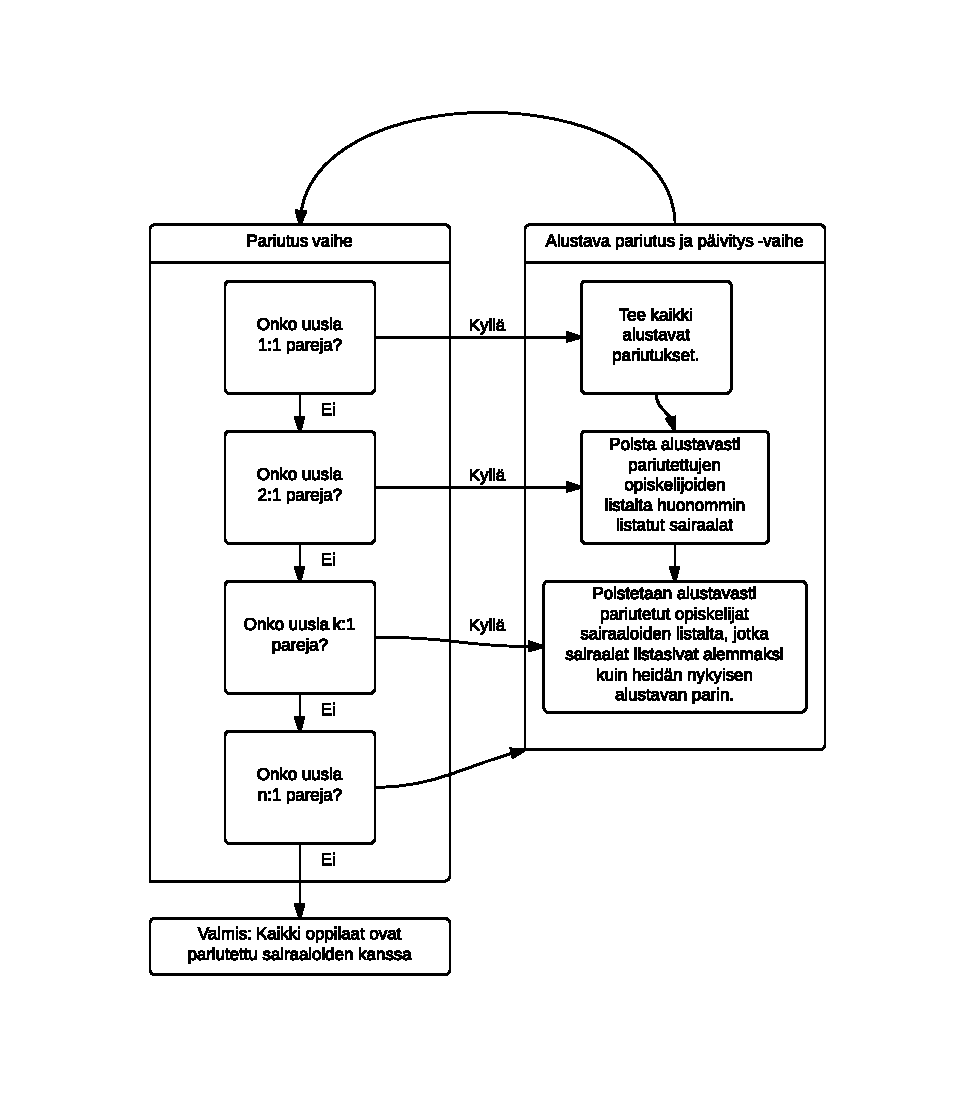
\includegraphics[scale=0.8]{NIMP}
\caption{Vuokaavio Algoritmistä \ref{nimp} \cite[s. 1009]{roth84}}
\label{nimp-vuo}
\end{figure}
Verrattuna Gale--Shapley-algoritmiin toimintaperiaate on hyvin erilainen ja monimutkainen ymmärtää, mutta molemmat tuottavat vakaita pariutuksia. Algoritmin \ref{nimp} pariutuksien vakauden todistus löytyy lähteestä ja se sivuutetaan tässä.

\section{Strategiat avioliittopeleissä}
Avioliittopeliin osallistuvan henkilön todelliset mieltymykset voivat hyvinkin erota hänen ilmoittamistaan mieltymyksistä. Mieltymykset mitkä henkilö julkisesti ilmoittaa kutsutaan strategiaksi \cite[s. 592]{Balinski}, joka muiden henkilöiden strategioiden kanssa koostavat vakaan pariutuksen kyseisessä avioliittopelissä.

Esimerkiksi olkoon olemassa nainen $n_1$, jonka aidot mieltymykset ovat seuraavat $m_1 > m_2 > m_3 > m_4$, pelistä ja miesten mieltymyksistä riippuen naisen on mahdollista päättyä kaikkien miesten kanssa avioliittoon. Jos nainen ilmoittaa mieltymyksikseen $m_1 > m_2$, ja ei edes harkitse avioliittoa miesten $m_3$ ja $m_4$ kanssa paranee naisen tilanne selvästi, ja avioliittopelissä hänen on mahdollista päätyä avioliittoon vain miehen $m_1$ tai $m_2$ kanssa.

Seuraavaksi näytetään, että rehellisyys on pätevä strategia, mutta mieltymysten muuntamisella voidaan saada henkilölle parempia pareja. Täytyy huomauttaa, että strategia on hyväksyttävä vain avioliittopeleissä joissa hyväksytään parien kieltäminen.

$\Gamma$ edustaa todellista mieltymyslistaa, joukko $M'$ miehiä, jotka väärentelevät mieltymyksiään ja $\Gamma'$ mieltymyslistaa, joka ottaa nämä väärennetyt mieltymykset huomioon $M_0$ on mies-optimaalinen pariutus suhteessa todellisiin mieltymyksiin $\Gamma$. 

\begin{lem}\cite[s. 55]{gusfield1989stable}\label{strategy-blocking}
	Olkoon $\mu$ pariutus ja oletetaan, että miesten joukko $\mathcal{X}$, jotka suosivat parejaan pariutuksessa $\mu$ kuin pariutuksessa $M_0$, ei ole tyhjä. Siinä tapauksessa on olemassa mies $m \notin \mathcal{X}$ ja nainen $n$ joka on estepari pariutuksella $\mu$
\end{lem}

\begin{proof}\cite[s. 55]{gusfield1989stable}\label{strategy-blockingtod}
	Pariutus $\mu$ on epävakaa, koska on olemassa miehiä jotka suosivat sitä enemmän kuin pariutusta $M_0$, joten jonkin parin on estettävä $\mu$. Näytetään, että jokin mies joka kuuluu joukkoon $\mathcal{X}$ on estävässä parissa. Olkoon $\mathcal{Y}$ joukko naisia, jotka ovat pareja miesten $\mathcal{X}$ kanssa pariutuksessa $M_0$. Todistus on jaettu kahteen tapaukseen.
	
	Ensimmäisessä tapauksessa oletetaan, että on olemassa mies $m'$ joukosta $\mathcal{X}$, joka on pariutettu naiseen $n$ joka ei ole joukosta $\mathcal{Y}$ pariutuksessa $\mu$. Koska $m'$ suosii paria $n$ verrattuna pariinsa pariutuksessa $M_0$, pariutus $M_0$ implikoi, että $n$ suosii $p_{M_0}(n)$ enemmän kuin $m'$. Mutta $n \notin \mathcal{Y}$ implikoi, että $m \notin \mathcal{X}$ ja $p_\mu(m) != n$, joten $m$ suosii naista $n$ enemmän kuin $p_\mu(m)$. Näin ollen, ensimmäisessä tapauksessa, $m$ ja $n$ estävät pariutuksen $\mu$ ja $m \notin \mathcal{X}$.
	
	Toisessa tapauksessa oletetaan, että jokainen mies joukosta $\mathcal{X}$ on pariutettu parituuksessa $\mu$ naisen kanssa joukosta $\mathcal{Y}$. Pariutuksen $M_0$ vakauden takia jokainen nainen joukosta $\mathcal{Y}$ suosii pariaan pariutuksessa $M_0$ verrattuna pariutukseen $\mu$. Missä tahansa mielivaltaisessa Gale--Shapley-algoritmin suorituksessa, jokainen tälläinen yllä kuvattu nainen hylkää $\mu$-parinsa. Oletetaan, että jossain mielivaltaisessa Gale--Shapley-algoritmin suorituksessa $m'$ on viimeinen mies joukosta $\mathcal{X}$, joka tekee kosinnan, olkoon $n$ nainen jota tämä $m'$ kosii. Nyt $n = p_{M_0}(m')$, joten $n$ on joukossa $\mathcal{Y}$. Koska $n$ hylkäsi miehen $p_\mu(n)$ algoritmin suorituksen aikana, on naisella $n$ oltava jokin mies langan päässä, esimerkiksi mies $m$, kun $m'$ kosii häntä. Nainen $n$ hylkää miehen $m$ ja hyväksyy miehen $m'$ ja koska $m$ jatkaa kosimalla ei se ole joukossa $\mathcal{X}$. Määritelmän mukaisesti $m$ ei suosi pariaan pariutuksessa $\mu$ verrattuna pariinsa pariutuksessa $M_0$, joten $m$ suosii naista $n$ enemmän kuin $p_\mu(m)$.
	
	Samoin koska $m \notin \mathcal{X}$ on viimeinen mies, joka hylätään naisen $n$ toimesta, suorituksen aikana jolloin tuotetaan pariutus $M_0$, ja $n \in \mathcal{Y}$ hylkäsi $p_\mu(n) \in \mathcal{X}$ suorituksen aikana, niin $n$ suosii miestä $m$ enemmän kuin miestä $p_\mu(n)$. Näin ollen kaksikko $m$ ja $n$ estävät pariutuksen $\mu$ ja $m \notin \mathcal{X}$, kuten haluttiin.	
\end{proof}

\begin{lau}\cite[s. 593]{Balinski}
	Oletetaan, että $\Gamma$ edustaa jokaisen henkilön aitoa mieltymystä ja $\Gamma'$ samoin, paitsi miesten $M'$ osajoukon, joilla on vaihtoehtoinen mieltymys $\Gamma'$:ssa. Ei ole olemassa vakaata pariutusta $\mu'$ $\Gamma'$:ssa jota kaikki miehet pitäisivät parempana kuin pariutusta $\mu$.
\end{lau}
\begin{proof}
	Oletetaan, että pariutus $\mu$ on miellyttävämpi kuin pariutus $\mu'$ miehille $m \in M' \subset M$. Lemman \ref{strategy-blocking} mukaan täytyy olla olemassa pari $m$ ja $n$ missä $m \notin M'$, joka estää pariutuksen $\mu$ mieltymyksillä $\Gamma$. Mutta miehen $m$ ja naisen $n$ strategiat ovat identtiset joukoissa $\Gamma$ ja $\Gamma'$, joten $m$ ja $n$ on estepari myös mieltymyksellä $\Gamma'$.
\end{proof}

Monessa avioliittopelissä tuloksia voidaan muunnella strategioilla vain silloin kun jokin osajoukko henkilöistä vääristelee yhdessä mieltymyksiä, eli he muodostavat \emph{koalition} ja tuottavat itselleen ja koalitiolle parempia pariutuksia.

\begin{lau}\cite[s. 58]{gusfield1989stable}
	Vaikka käytetään nais-orientoitunutta Gale--Shapley-algoritmiä (naiset kosii, miehet päättää), voivat miehet pakottaa algoritmin tuottamaan mies-optimaalisia tuloksia antamalla väärennettyjä mieltymyksiä.
\end{lau}

\begin{proof}
	Jokainen mies $m$ väärentää mieltymyslistansa. Nämä miehet ilmoittavat, että huonompi nainen kuin $p_{M_0}(m)$ on hylättävä ja ei sovi miehelle pariksi, tämä tuottaa mieltymslistan $\Gamma'$. Jos mies-orientoitunutta Gale--Shapley-algoritmiä käytetään mieltymyksille $\Gamma'$ se tuottaa $M_0$, mies-optimaalisen pariutuksen mieltymyksille $\Gamma$. Edelleen, koska pariutuksessa $M_0$ jokaisella miehellä on huonoin mahdollinen pari suhteessa mieltymyslistaan $\Gamma'$, on se ainoa mahdollinen vakaa pariutus tässä kontekstissa. Näin ollen $M_0$ on vakaa pariutus jonka nais-orientoitunut Gale--Shapley-algoritmi tuottaa suhtessa mieltymyksiin $\Gamma'$.
\end{proof}

Ylläolevalla strategialla on eräs vakaus ominaisuus joka rohkaisee miehiä toteuttamaan sovittu strategia. Oletetaan, että miehet sopivat keskenään ylläolevan kaltaisesta strategiasta, mutta ennen kuin väärennetty mieltymyslista julkaistaan jokin osajoukko koalitiosta päättää pettää koalition. Nämä miehet olettavat, että loput koalition miehet toteuttavat alkuperäisen strategian ja naiset antavat todelliset mieltymyksensä. Ongelmana pettäjillä on löytää optimoitu mieltymyslista, joka tuottaa heille vielä parempia pareja. Vaikka tälläistä petosta ei tapahtuisi jokainen mies voi olla huolissaan, että tälläinen petos tapahtuu hänen selkänsä takana ja epäröi osallistumistaan alkuperäiseen strategiaan, jossa kaikki miehet antoivat väärennetyt mieltymyslistat. Seuraava lause kertoo, että koalition on turha etsiä parempaa strategiaa ja näin ollen miesten ei tarvitse huolehtia petoksista koalitioissa \cite{gusfield1989stable}.

\begin{lem}\cite[s. 56]{gusfield1989stable}\label{strategy-gus}
	Ei ole olemassa vakaata pariutuksia suhteessa mieltymyksiin $M'$, missä jokainen mies joukosta $M'$ saa parin jota suosii ehdottomasti enemmän kuin pariaan pariutuksessa $M_0$.
\end{lem}

\begin{proof}\cite[s. 56]{gusfield1989stable}
	Olkoon $\mu$ pariutus missä jokin joukko miehiä $M' \supseteq M$ saavat parit joita he suosivat enemmän kuin parejaan pariutuksessa $M_0$. Lemman \ref{strategy-blocking} mukaan on olemassa kaksikko $m$ ja $n$, joka estää pariutuksen $\mu$ suhteessa mieltymyksiinn $\Gamma$, niin että $m$ ei ole joukossa $M'$. Mutta nyt $m$ ei ole joukossa $M$, joten $\Gamma'$ sisältää molempien, miehen $m$ ja naisen $n$, todelliset mieltymykset, ja näin ollen heidän on estettävä pariutus $\mu$ myös suhteessa mieltymyksiin $\Gamma'$. Joten ei ole olemassa vakaata pariutusta missä jokainen mies joukosta $M$ parantaisi hänen pariaan verrattuna pariutukseen $M_0$. 
\end{proof}

\begin{lau}\cite[s. 58]{gusfield1989stable}
	Olkoon $M'$ miesten osajoukko ja olkoon $\mu$ mikä tahansa pariutus missä jokainen mies joukosta $M'$ suosii $\mu$-pariaan enemmän kuin $M_0$-pariaan. Olettaen, että jokainen mies joka ei ole joukossa $M'$ ilmoittaa hänen $\Gamma'$ listansa, ja jokainen nainen ilmoittaa heidän $\Gamma$ listansa, ei ole olemassa sellaista listojen joukkoja minkä $M'$ voi ilmoittaa niin että $\mu$ olisi vakaa suhteessa ilmoitettuihin listoihin.
\end{lau}

\begin{proof}
	Oletetaan, että jokin osajoukko joukosta $M'$ väärentää heidän sovitut mieltymyslistat luomalla mieltymykset $\Gamma_{M'}$ aikaisemman ja sovitun $\Gamma'$ mieltymyslistan sijaan. Nyt $M_0$ on ainoa vakaa pariutus mieltymyksille $\Gamma'$, joten se on siis mies-optimaalinen pariutus molemmissa $\Gamma$:ssa ja $\Gamma'$:ssa. Näin ollen jos miehet joukossa $M'$ parantelevat parejaan, suhteessa mieltymyksiin $\Gamma$, petoksen johdosta on kaikkien heidän saatava paremmat parit verrattuna mies-optimaaliseen pariutukseen mieltymyksillä $\Gamma'$. Mutta lemma \ref{strategy-gus} nojalla miesten joukossa $M'$ on mahdotonta ehdottomasti parantaa pariaan mieltymyksilla $\Gamma'$ valehtelemalla.
\end{proof}


% --- Back matter ---
%
% bibtex is used to generate the bibliography. The babplain style
% will generate numeric references (e.g. [1]) appropriate for theoretical
% computer science. If you need alphanumeric references (e.g [Tur90]), use
%
% \bibliographystyle{babalpha-lf}
%
% instead.

\bibliographystyle{babplain-lf}
\bibliography{ref}


\end{document}
